\chapter*{Appendix}
\label{appendix}
% Following is required as above uses \chapter*{} (note the star). The start makes the chapter unnumbered, but also removes it from table of content. Former is desired, the latter is not:
\addcontentsline{toc}{chapter}{Appendix}

Various statistical methods were tested to detect outlier nodes. The impact of removing
these nodes is illustrated in the plots from \fref{fig:std_dv_plots} to
\fref{fig:top20_plots} and \fref{tab:outlier_detection_methods} . below.

\begin{figure}[h]
	\centering
	\subfloat[Community Sizes Comparison (Standard Deviation)]{%
	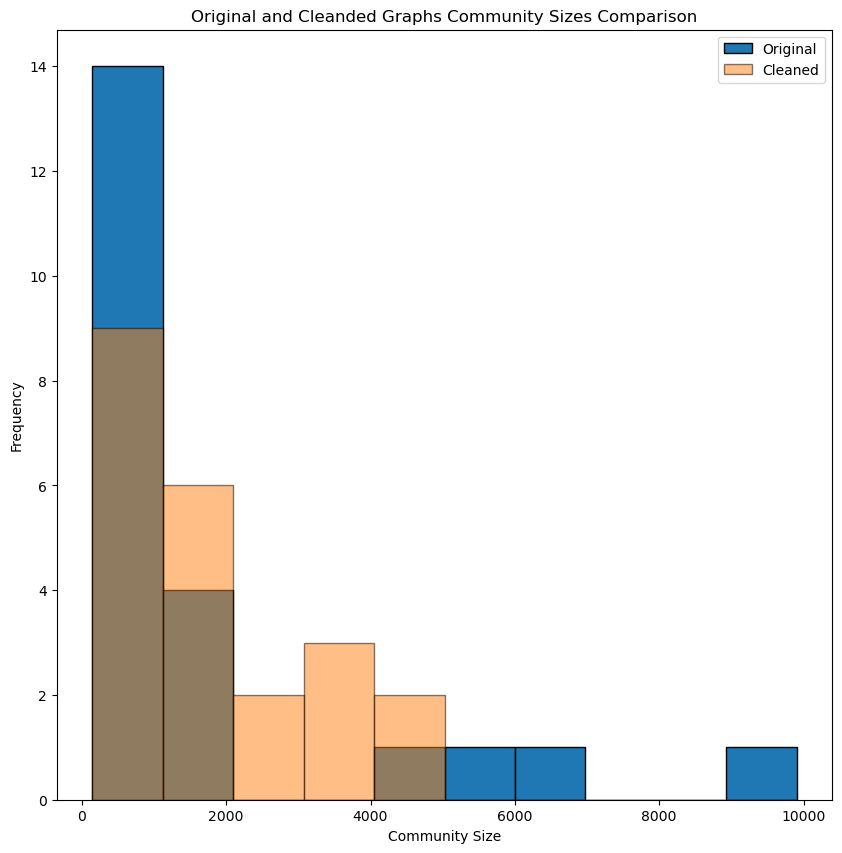
\includegraphics[width=0.45\textwidth]{images/Appendix_A/std_dv_community_sizes_comparison.png} \label{fig:std_dv_community_sizes_comparison} }
	\hfill \subfloat[Degree Centrality Distribution of Removed Nodes (Standard
	Deviation)]{%
	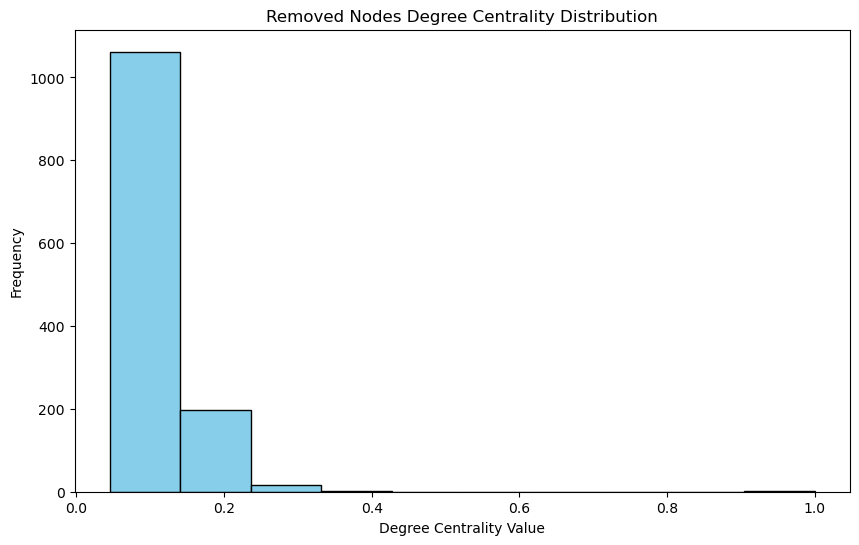
\includegraphics[width=0.45\textwidth]{images/Appendix_A/std_dv_removed_nodes_degree_centrality_distribution.png} \label{fig:std_dv_removed_nodes_degree_centrality_distribution} }
	\caption{Comparison of Community Sizes and Degree Centrality Distribution of
	Removed Nodes Using the Standard Deviation Method}
	\label{fig:std_dv_plots}
\end{figure}

\begin{figure}[h]
	\centering
	\subfloat[Community Sizes Comparison (Percentile)]{%
	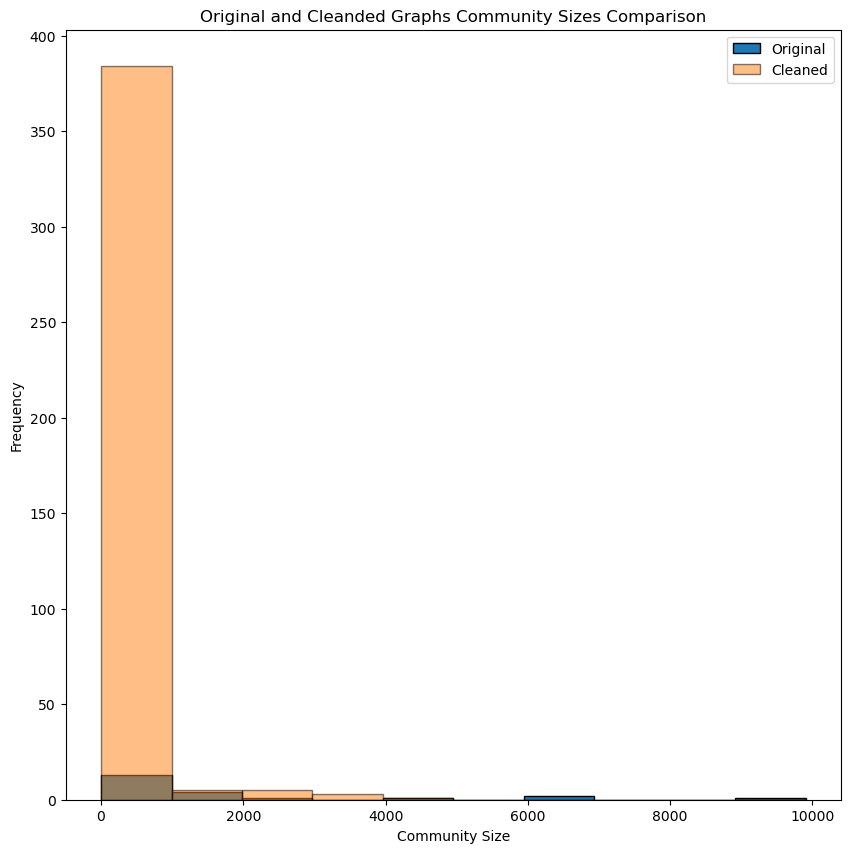
\includegraphics[width=0.45\textwidth]{images/Appendix_A/percentile_community_sizes_comparison.png} \label{fig:percentile_community_sizes_comparison} }
	\hfill \subfloat[Degree Centrality Distribution of Removed Nodes (Percentile)]{%
	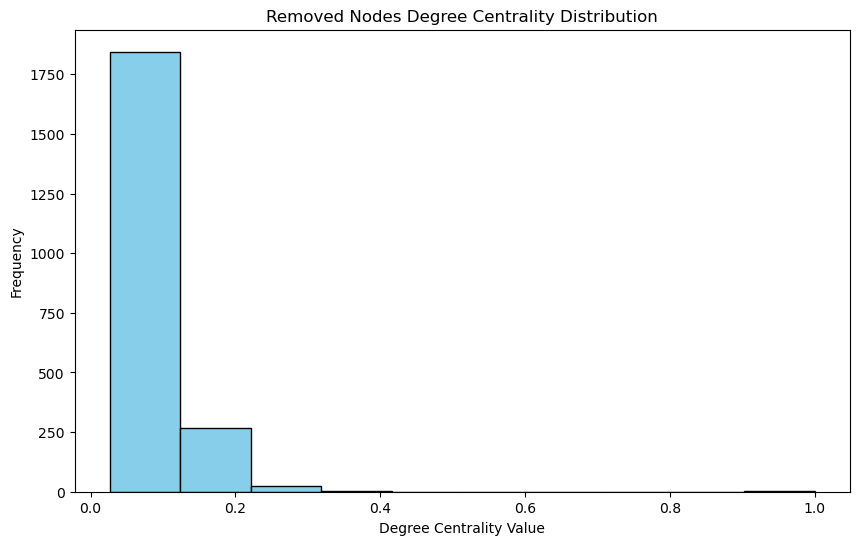
\includegraphics[width=0.45\textwidth]{images/Appendix_A/percentile_removed_nodes_degree_centrality_distribution.png} \label{fig:percentile_removed_nodes_degree_centrality_distribution} }
	\caption{Comparison of Community Sizes and Degree Centrality Distribution of
	Removed Nodes Using the Percentile Method}
	\label{fig:percentile_plots}
\end{figure}

\begin{figure}[h]
	\centering
	\subfloat[Community Sizes Comparison (IQR)]{%
	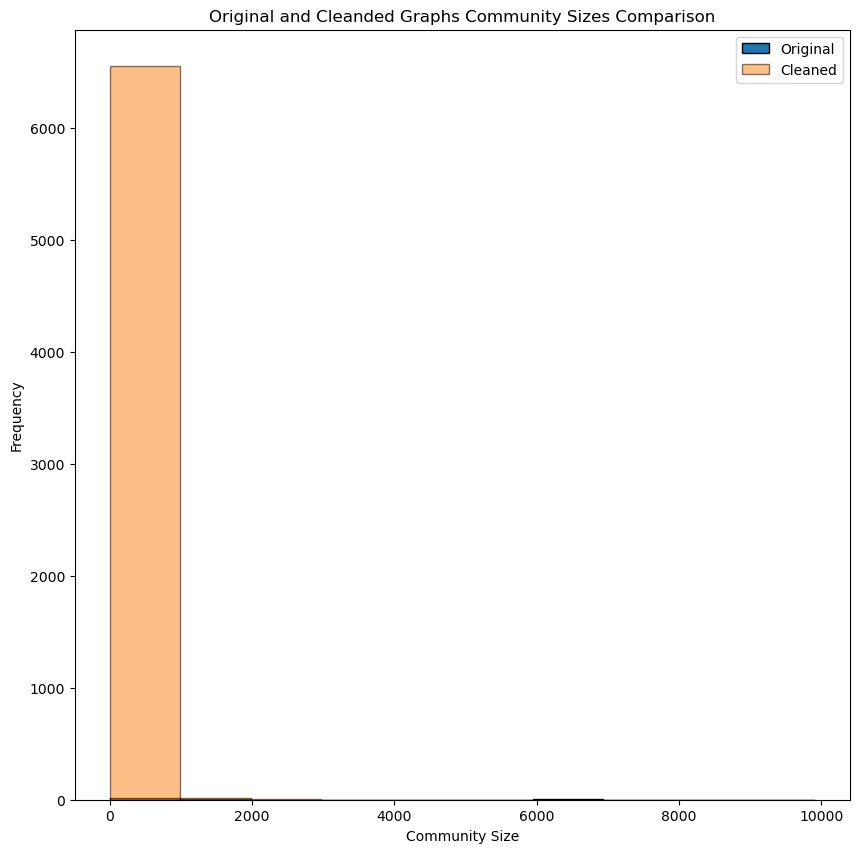
\includegraphics[width=0.45\textwidth]{images/Appendix_A/IQR_community_sizes_comparison.png} \label{fig:IQR_community_sizes_comparison} }
	\hfill \subfloat[Degree Centrality Distribution of Removed Nodes (IQR)]{%
	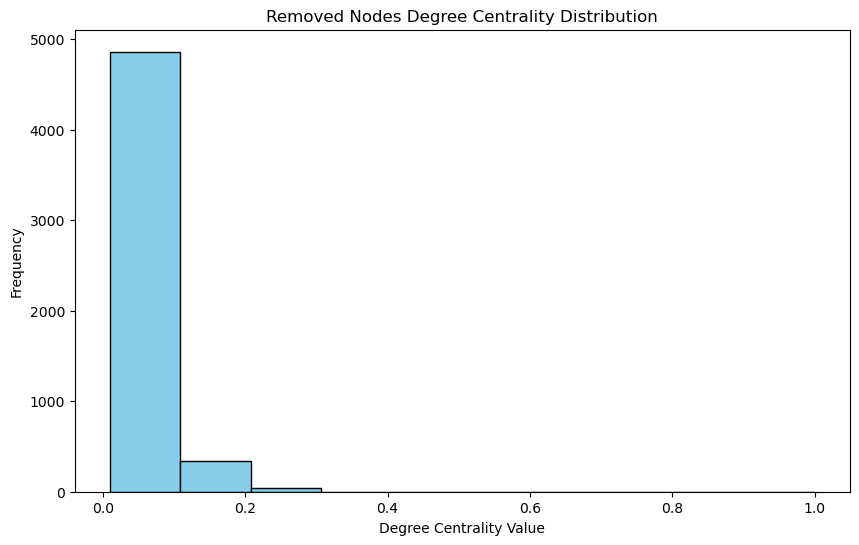
\includegraphics[width=0.45\textwidth]{images/Appendix_A/IQR_removed_nodes_degree_centrality_distribution.png} \label{fig:IQR_removed_nodes_degree_centrality_distribution} }
	\caption{Comparison of Community Sizes and Degree Centrality Distribution of
	Removed Nodes Using the IQR Method}
	\label{fig:IQR_plots}
\end{figure}

\begin{figure}[h]
	\centering
	\subfloat[Community Sizes Comparison (Knee Method)]{%
	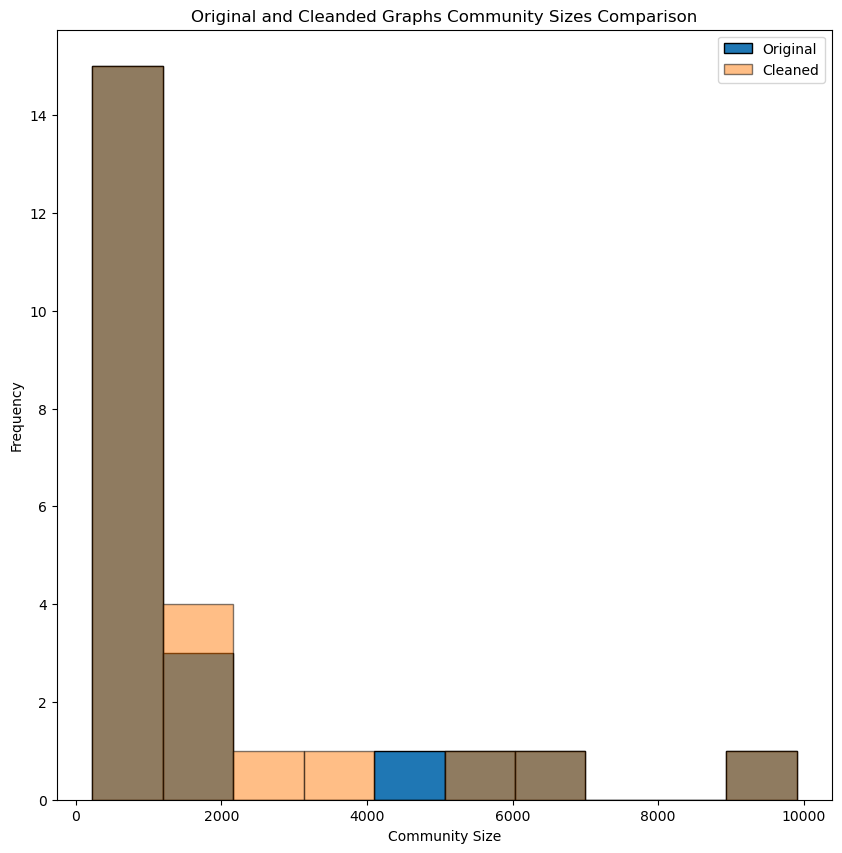
\includegraphics[width=0.45\textwidth]{images/Appendix_A/knee_community_sizes_comparison.png} \label{fig:knee_community_sizes_comparison} }
	\hfill \subfloat[Degree Centrality Distribution of Removed Nodes (Knee Method)]{%
	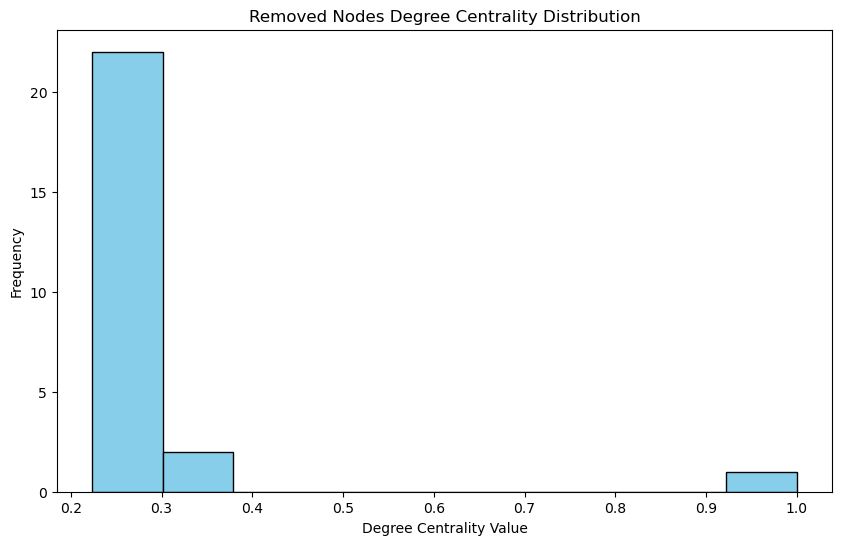
\includegraphics[width=0.45\textwidth]{images/Appendix_A/knee_removed_nodes_degree_centrality_distribution.png} \label{fig:knee_removed_nodes_degree_centrality_distribution} }
	\caption{Comparison of Community Sizes and Degree Centrality Distribution of
	Removed Nodes Using the Knee Method}
	\label{fig:knee_plots}
\end{figure}

\begin{figure}[h]
	\centering
	\subfloat[Community Sizes Comparison (Top 20 Method)]{%
	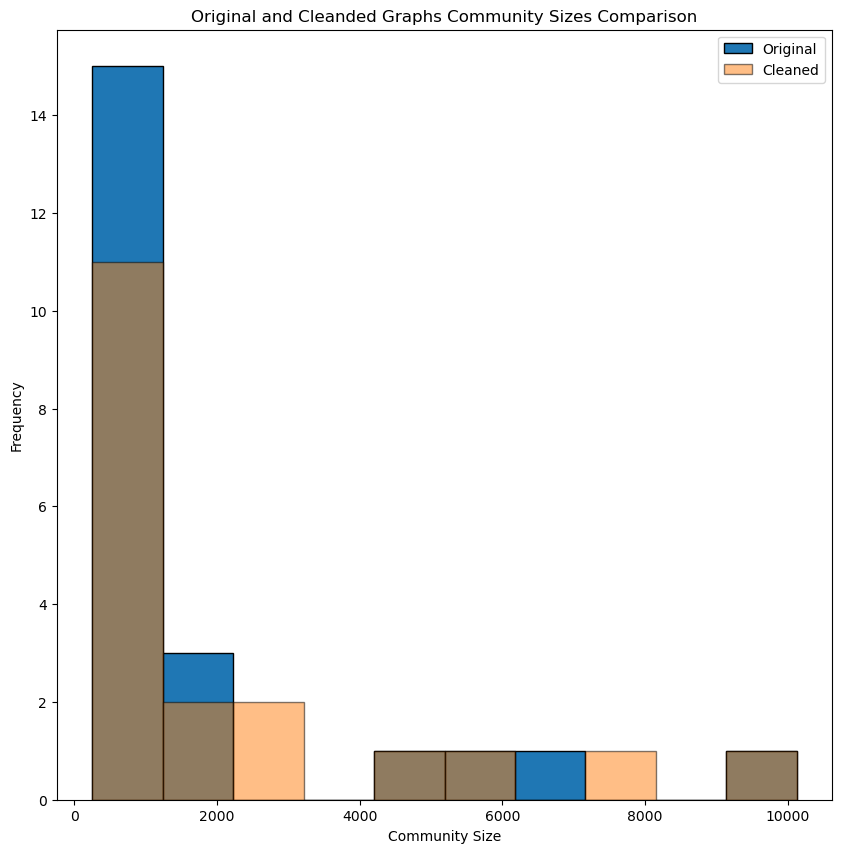
\includegraphics[width=0.45\textwidth]{images/Appendix_A/top20_community_sizes_comparison.png} \label{fig:top20_community_sizes_comparison} }
	\hfill \subfloat[Degree Centrality Distribution of Removed Nodes (Top 20
	Method)]{%
	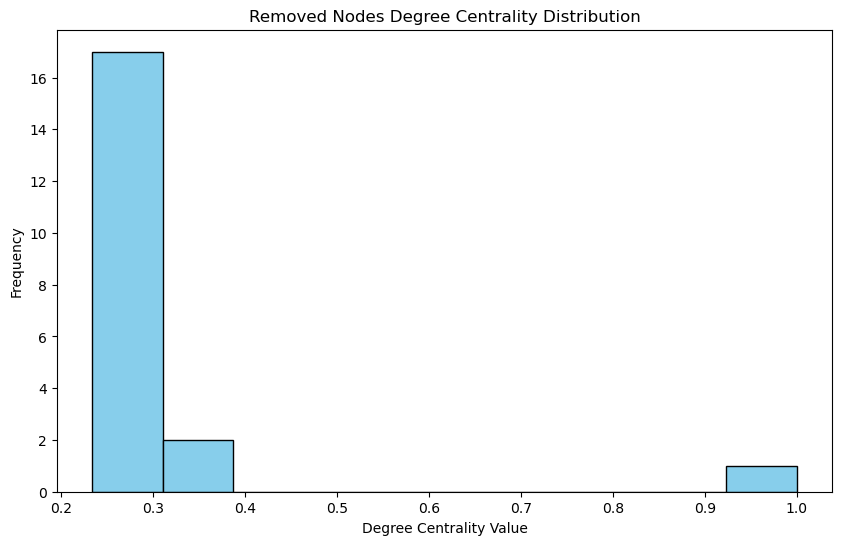
\includegraphics[width=0.45\textwidth]{images/Appendix_A/top20_removed_nodes_degree_centrality_distribution.png} \label{fig:top20_removed_nodes_degree_centrality_distribution} }
	\caption{Comparison of Community Sizes and Degree Centrality Distribution of
	Removed Nodes Using the Top 20 Method}
	\label{fig:top20_plots}
\end{figure}


\clearpage
\begin{table}[h]
	\centering
	\begin{adjustbox}
		{width=1.1\textwidth, center}
		\begin{tabular}{l c c c}
			\hline
			\textbf{Method/Metric} & \textbf{\# of Removed Nodes} & \textbf{\# Nodes in Cleaned Graph} & \textbf{\# of Communities in Cleaned Graph} \\
			\hline
			Standard Deviation     & 1279                         & 41391                              & 22                                          \\
			IQR                    & 5241                         & 37429                              & 6559                                        \\
			Percentile             & 2137                         & 40533                              & 398                                         \\
			Knee Method            & 25                           & 42645                              & 24                                          \\
			Top 20                 & 20                           & 42650                              & 19                                          \\
			\hline
		\end{tabular}
	\end{adjustbox}
	\caption{Comparison of Outlier Detection Methods}
	\label{tab:outlier_detection_methods}
\end{table}